\chapter{Status of the application}

% geoserver running
% database working
% able to do queries (getcapabilities, getfeatureofinterest)
% unable to query the actual data
% kvp works, JSON doesn't

The application that was created during the course of this project is almost finished. The steps that needed to be taken to get from the raw Wi-Fi data to the SOS on the geoserver have all been taken, but some debugging is still to be done to have a final working application. \\

Setting up the geoserver was the easy part. The webapp that 52°North provided
could be imported directly into the geoserver running on the local machines. The
configuration of the 52°North SOS was slightly harder. The original Wi-Fi
tracking data is on a remote server on the TU Delft campus, but the encoding for
that server is in 'LATIN1', which is unsupported by the 52°North SOS. It required a new database with UTF-8 encoding to get the SOS tables in the database. Filling the tables with the tracking data took most of the time, but using the 52°North application as a guide ensured that the correct attributes were used in the tables. \\

Finally, the 52°North webapp could be used to do sample queries on the database to check if the database model was correct. This worked and showed that the database model was correct. \autoref{figure:testqueries} shows such a sample query and the result from the database. 
\begin{figure}[H]
\centering
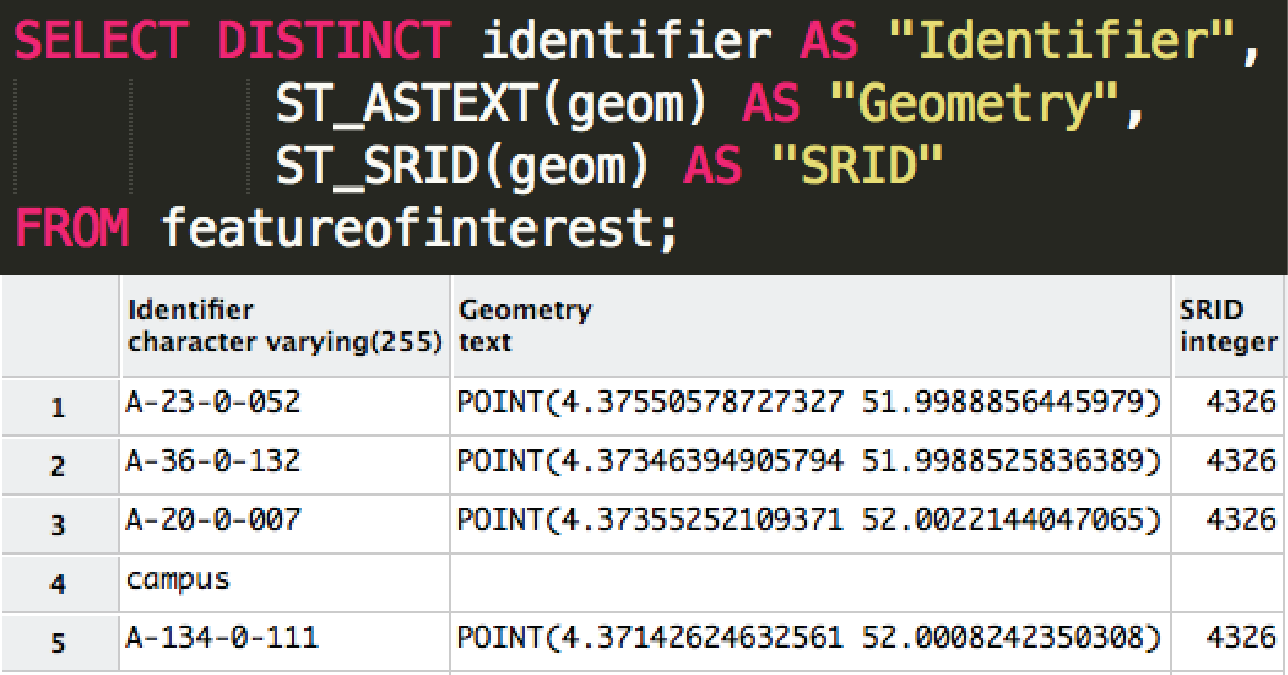
\includegraphics[scale=0.8]{testqueries.png}
\captionsetup{justification=centering}
\caption{Test queries on the database}
\label{figure:testqueries}
\end{figure}

Additionally, sample requests can also be sent. These sample requests can be
generated by the 52°North webapp test client. Such requests are
\textit{GetCapabilities} and \textit{GetFeatureOfInterest}. The screenshots of
these requests are depicted in appendix A. \\

From the bindings that are available to send the request (JSON, KVP, SOAP and POX), only the KVP (Key Value Pairs) seemed to work. Unfortunately the other bindings would result in errors. Without deeper understanding about SOS and these bindings, we were not able to debug the errors and create valid requests. 

Furthermore, we were able the retrieve the observations with KVP binding and
\textit{GetObservation} procedure, using the extension
\textit{MergeObservationsIntoDataArray}. This procedure returnes the
\textit{description, type, phenomenonStartTime, phenomenonEndTime, 
resultTime, procedure identifier and name, observedProperty identifier and 
name, result and the type, name, identifier, coordinates of the 
featureOfInterest}. See the request below and a screenshot of the result in the 
appendix.

\url{http://localhost:8080/52n-sos-webapp/service?service=SOS&version=2.0.0&request=GetObservation&MergeObservationsIntoDataArray=true&procedure=wifi_access_point}

However, the same request without using the extension returns an empty result,
no error message. See the url below.

\url{http://localhost:8080/52n-sos-webapp/service?service=SOS&version=2.0.0&request=GetObservation&procedure=wifi_access_point}
